\subsection{Frozen representations recover anatomy in held-out sections}
\label{sec:dual-view-identification}

Frozen ZoomST representations distinguish anatomical compartments on sections excluded from pretraining. We compare whole-section clustering with atlas annotations across all eight held-out MOSTA sections. Molecular features concatenate $e_8,e_{32},e_{128}$, spatial features concatenate $g_8,g_{32},g_{128}$, and joint features combine both views. All pretrained encoders remain frozen; the target-section readouts are specified in Appendix~\ref{app:dual-view}.

Joint ZoomST features achieve higher AMI than the evaluated public pretrained baselines on every held-out section, with an equal-section mean of 0.577, and remain competitive with target-fitted spatial methods (Table~\ref{tab:representation-summary}). The same features retain 52.7\% of physical 32-nearest neighbors on average, linking anatomical agreement to local spatial organization. The matched-update No Cross model has similar mean AMI (0.575), but lower neighbor retention (50.4\%). Thus, the full model retains anatomical discrimination while improving local spatial correspondence relative to this ablation.

\begin{table}[!htbp]
\centering\small
\caption{\textbf{Tissue mapping and neighbor retention on eight held-out MOSTA sections.} \textbf{(a)} AMI as mean $\pm$ sample SD over clustering seeds 42, 43, and 44; the summary averages sections equally within each seed. \textbf{(b)} Equal-section mean recovery of physical 32-nearest neighbors. Molecular and Spatial Views each concatenate three granularities; Joint combines both. No Cross uses the same joint readout and total training updates without cross-granularity supervision. Pretrained encoders are frozen. Bold marks the top three unrounded values per row, including third-place ties. Protocol: Appendix~\ref{app:dual-view}.}
\label{tab:representation-summary}
\label{tab:dual-view-sections}
\setlength{\tabcolsep}{0.8pt}
\renewcommand{\arraystretch}{1.05}
\begin{tabular}{lcccccccccc}
\toprule
 & \multicolumn{4}{c}{ZoomST Versions} & \multicolumn{2}{c}{Frozen pretrained} & \multicolumn{4}{c}{Target-fitted} \\
\cmidrule(lr){2-5}\cmidrule(lr){6-7}\cmidrule(lr){8-11}
Stage & Joint & \shortstack{Molecular\\View} & \shortstack{Spatial\\View} & \shortstack{No Cross\\Ablation} & Novae & SToFM & GraphST & BANKSY & MENDER & STAGATE \\
\midrule
\multicolumn{11}{l}{\textbf{(a) Anatomical agreement: AMI} $\uparrow$} \\
E9.5 & \textbf{0.547} & 0.486 & \textbf{0.556} & 0.533 & 0.371 & 0.211 & 0.538 & 0.540 & 0.530 & \textbf{0.556} \\
 & {\scriptsize $\pm 0.014$} & {\scriptsize $\pm 0.016$} & {\scriptsize $\pm 0.017$} & {\scriptsize $\pm 0.005$} & {\scriptsize $\pm 0.007$} & {\scriptsize $\pm 0.004$} & {\scriptsize $\pm 0.009$} & {\scriptsize $\pm 0.021$} & {\scriptsize $\pm 0.005$} & {\scriptsize $\pm 0.028$} \\
\addlinespace[2pt]
E10.5 & \textbf{0.549} & 0.516 & 0.534 & \textbf{0.549} & 0.390 & 0.262 & 0.534 & 0.539 & 0.531 & \textbf{0.544} \\
 & {\scriptsize $\pm 0.009$} & {\scriptsize $\pm 0.014$} & {\scriptsize $\pm 0.002$} & {\scriptsize $\pm 0.004$} & {\scriptsize $\pm 0.004$} & {\scriptsize $\pm 0.013$} & {\scriptsize $\pm 0.010$} & {\scriptsize $\pm 0.013$} & {\scriptsize $\pm 0.001$} & {\scriptsize $\pm 0.023$} \\
\addlinespace[2pt]
E11.5 & \textbf{0.628} & \textbf{0.608} & \textbf{0.615} & 0.602 & 0.444 & 0.291 & 0.502 & 0.573 & 0.561 & 0.559 \\
 & {\scriptsize $\pm 0.001$} & {\scriptsize $\pm 0.004$} & {\scriptsize $\pm 0.010$} & {\scriptsize $\pm 0.001$} & {\scriptsize $\pm 0.008$} & {\scriptsize $\pm 0.007$} & {\scriptsize $\pm 0.004$} & {\scriptsize $\pm 0.022$} & {\scriptsize $\pm 0.002$} & {\scriptsize $\pm 0.007$} \\
\addlinespace[2pt]
E12.5 & \textbf{0.613} & \textbf{0.614} & 0.607 & \textbf{0.618} & 0.447 & 0.307 & 0.509 & 0.583 & 0.582 & 0.585 \\
 & {\scriptsize $\pm 0.015$} & {\scriptsize $\pm 0.003$} & {\scriptsize $\pm 0.006$} & {\scriptsize $\pm 0.013$} & {\scriptsize $\pm 0.011$} & {\scriptsize $\pm 0.008$} & {\scriptsize $\pm 0.017$} & {\scriptsize $\pm 0.007$} & {\scriptsize $\pm 0.009$} & {\scriptsize $\pm 0.017$} \\
\addlinespace[2pt]
E13.5 & \textbf{0.578} & 0.541 & \textbf{0.579} & 0.573 & 0.432 & 0.334 & 0.386 & \textbf{0.593} & 0.573 & 0.544 \\
 & {\scriptsize $\pm 0.012$} & {\scriptsize $\pm 0.011$} & {\scriptsize $\pm 0.012$} & {\scriptsize $\pm 0.003$} & {\scriptsize $\pm 0.003$} & {\scriptsize $\pm 0.017$} & {\scriptsize $\pm 0.013$} & {\scriptsize $\pm 0.015$} & {\scriptsize $\pm 0.009$} & {\scriptsize $\pm 0.006$} \\
\addlinespace[2pt]
E14.5 & 0.563 & 0.556 & 0.558 & \textbf{0.571} & 0.450 & 0.407 & 0.453 & \textbf{0.572} & 0.535 & \textbf{0.579} \\
 & {\scriptsize $\pm 0.019$} & {\scriptsize $\pm 0.009$} & {\scriptsize $\pm 0.006$} & {\scriptsize $\pm 0.017$} & {\scriptsize $\pm 0.009$} & {\scriptsize $\pm 0.006$} & {\scriptsize $\pm 0.005$} & {\scriptsize $\pm 0.008$} & {\scriptsize $\pm 0.004$} & {\scriptsize $\pm 0.021$} \\
\addlinespace[2pt]
E15.5 & \textbf{0.626} & \textbf{0.625} & 0.614 & \textbf{0.630} & 0.494 & 0.405 & 0.422 & 0.614 & 0.600 & 0.604 \\
 & {\scriptsize $\pm 0.001$} & {\scriptsize $\pm 0.006$} & {\scriptsize $\pm 0.004$} & {\scriptsize $\pm 0.013$} & {\scriptsize $\pm 0.004$} & {\scriptsize $\pm 0.005$} & {\scriptsize $\pm 0.005$} & {\scriptsize $\pm 0.003$} & {\scriptsize $\pm 0.010$} & {\scriptsize $\pm 0.003$} \\
\addlinespace[2pt]
E16.5 & 0.513 & 0.497 & \textbf{0.532} & 0.524 & 0.449 & 0.331 & 0.403 & \textbf{0.526} & 0.509 & \textbf{0.540} \\
 & {\scriptsize $\pm 0.010$} & {\scriptsize $\pm 0.012$} & {\scriptsize $\pm 0.007$} & {\scriptsize $\pm 0.008$} & {\scriptsize $\pm 0.006$} & {\scriptsize $\pm 0.007$} & {\scriptsize $\pm 0.002$} & {\scriptsize $\pm 0.006$} & {\scriptsize $\pm 0.016$} & {\scriptsize $\pm 0.006$} \\
\addlinespace[2pt]
Mean AMI & \textbf{0.577} & 0.555 & \textbf{0.574} & \textbf{0.575} & 0.435 & 0.319 & 0.468 & 0.567 & 0.553 & 0.564 \\
 & {\scriptsize $\pm 0.004$} & {\scriptsize $\pm 0.006$} & {\scriptsize $\pm 0.003$} & {\scriptsize $\pm 0.003$} & {\scriptsize $\pm 0.001$} & {\scriptsize $\pm 0.003$} & {\scriptsize $\pm 0.003$} & {\scriptsize $\pm 0.003$} & {\scriptsize $\pm 0.002$} & {\scriptsize $\pm 0.0005$} \\
\addlinespace[2pt]
\midrule
\multicolumn{11}{l}{\textbf{(b) Local spatial organization} $\uparrow$} \\
\shortstack{Neighbor\\retention} & \textbf{0.527} & 0.502 & \textbf{0.523} & \textbf{0.504} & 0.313 & 0.033 & 0.268 & 0.483 & 0.354 & 0.354 \\
\bottomrule
\end{tabular}

\end{table}

The held-out E16.5 E2S13 Brain case illustrates the complementary information in the two views (Figure~\ref{fig:dual-view-brain}). Molecular features recover most Brain positions but include neighboring tissue; spatial features make fewer extra assignments but miss part of the Brain. Joint features reduce this tradeoff, increasing Brain IoU from 0.884 for $e$ and 0.905 for $g$ to 0.962. Whole-section maps and section-wise spatial retention are provided in Figures~\ref{fig:dual-view-e125} and~\ref{fig:dual-view-retention}. These results establish a transferable representation base from which to assess the additional value of learning granularity relationships.

\begin{figure}[!htbp]
\centering
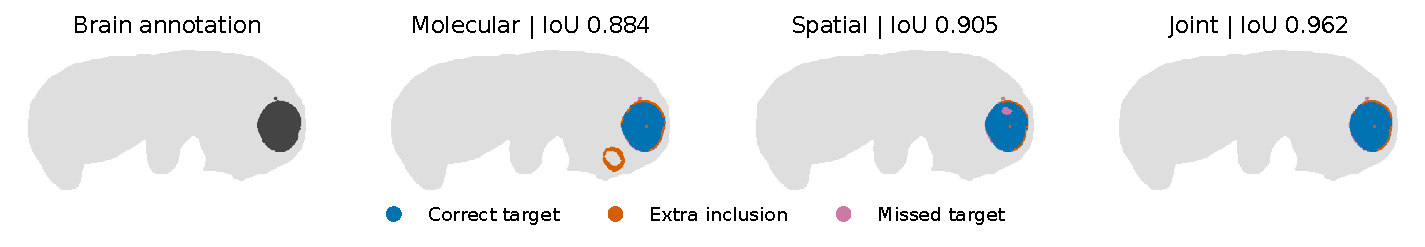
\includegraphics[width=\linewidth]{figures/brain_complementarity.pdf}
\caption{\textbf{Complementary molecular and spatial errors on a held-out section.} Annotation, molecular, spatial, and joint Brain assignments in E16.5 E2S13. Blue: correct assignments; orange: extra assignments; magenta: missed Brain. All maps use the same whole-section readout and seed 42. Each feature set combines its respective training granularities.}
\label{fig:dual-view-brain}
\end{figure}
\FloatBarrier
